\documentclass{article}
\usepackage{tikz}
\usetikzlibrary{calc}
\usepackage{amsmath}
\usepackage{amssymb}
\usepackage[margin=1in]{geometry}
\tikzset{
  v/.style={draw, circle, inner sep=0pt, font=\small, align=center, minimum size=0.75cm},
  e/.style={->, dashed}
}
\newcommand{\dottedarrow}[2]{\draw[e] ($(#1)!0.5cm!(#2)$) -> ($(#1)!1cm!(#2)$)}
\newcommand{\dottedarrows}[4]{
  \foreach \i in #1 {
    \foreach \j in #2 {
      \ifnum\pdfstrcmp{\i}{#3}=0
        \ifnum\pdfstrcmp{\j}{#4}=0
        \else
          \dottedarrow{\i}{\j};
        \fi
      \else
        \dottedarrow{\i}{\j};
      \fi
    }
  }
}
\begin{document}
\section{Complexity of reduced cases}
\subsection{Single course, single start date, single weekly pattern}

This case can be solved in polynomial time. Indeed, it is a simple case of a maximum-cost maximum-flow problem. Specifically, if we let \begin{itemize}
\item $p$ be the number of professors,
\item $d$ be the number of days,
\item $m$ be the number of roles, and
\item $n'_{i, k}$ be the number of professors of role $k$ that are needed on whichever class falls on the $i$th day
\end{itemize}

we can create the following flow network, where capacities are in blue, and costs are in red:

\vspace{10pt}

\begin{center}
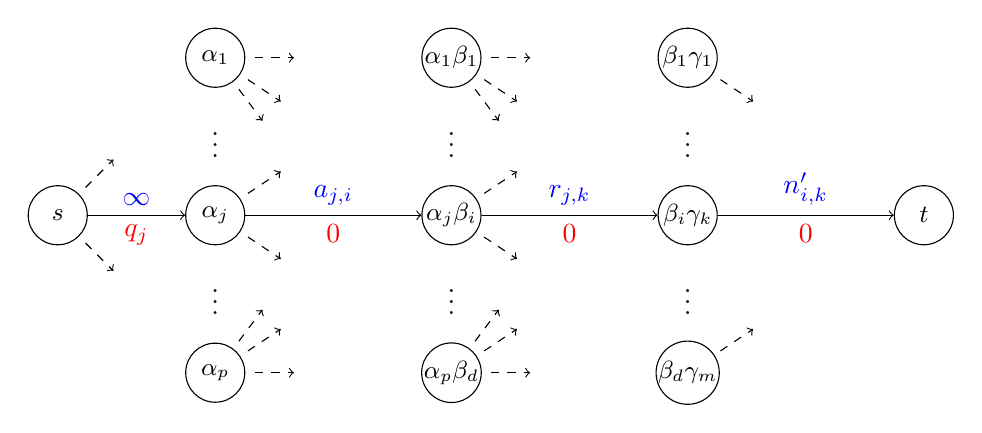
\begin{tikzpicture}

\tikzstyle{v}=[draw, circle, inner sep=0pt, font=\small, align=center, minimum size=0.75cm];
\tikzstyle{e}=[->, dashed];
\node[v] (s) at (1, 1) {$s$};
\node[v] (p_j) at (3, 1) {$\alpha_j$};
\node (d1) at (3, 2) {$\vdots$};
\node (d2) at (3, 0) {$\vdots$};
\node[v] (d3) at (3, 3) {$\alpha_1$};
\node[v] (d4) at (3, -1) {$\alpha_p$};

\node[v] (p_jd_i) at (6, 1) {$\alpha_j \beta_i$};
\node (d5) at (6, 0) {$\vdots$};
\node (d6) at (6, 2) {$\vdots$};
\node[v] (d7) at (6, 3) {$\alpha_1 \beta_1$};
\node[v] (d8) at (6, -1) {$\alpha_p \beta_d$};

\node[v] (d_ir_k) at (9, 1) {$\beta_i \gamma_k$};
\node (d9) at (9, 0) {$\vdots$};
\node (d10) at (9, 2) {$\vdots$};
\node[v] (d11) at (9, 3) {$\beta_1 \gamma_1$};
\node[v] (d12) at (9, -1) {$\beta_d \gamma_m$};

\node[v] (t) at (12, 1) {$t$};

\draw[->] (s) to node[above,blue] {$\infty$} node[below,red] {$q_j$} (p_j);

\dottedarrows{{s}}{{d3, d4}};

\draw[->] (p_j) to node[above,blue] {$a_{j, i}$} node[below,red] {$0$} (p_jd_i);

\dottedarrows{{d3, d4, p_j}}{{d7, p_jd_i, d8}}{p_j}{p_jd_i};

\draw[->] (p_jd_i) to node[above,blue] {$r_{j, k}$} node[below,red] {$0$} (d_ir_k);

\dottedarrows{{d7, d8, p_jd_i}}{{d11, d12, d_ir_k}}{p_jd_i}{d_ir_k};

\draw[->] (d_ir_k) to node[above,blue] {$n'_{i, k}$} node[below,red] {$0$} (t);

\dottedarrows{{d11, d12}}{{t}};

\end{tikzpicture}
\end{center}

Formally, the network is $G = (V, E)$, with

\begin{align*}
V = &\{s\} \cup \{t\}\\
&\cup \{\alpha_j \mid 1 \le j \le p\}\\
&\cup \{\alpha_j \beta_i \mid 1 \le j \le p, 1 \le i \le d\}\\
&\cup \{\beta_i \gamma_k \mid 1 \le i \le d, 1 \le j \le m\}\\
E = &\{(s, \alpha_j)\ \forall\ j\}\\
    &\cup \{(\alpha_j, \alpha_j \beta_i)\ \forall\ i, j \}\\
    &\cup \{(\alpha_j \beta_i, \beta_i \gamma_k)\ \forall\ j, i, k\}\\
    &\cup \{(\beta_i \gamma_k, t)\ \forall\ i, k \}
\end{align*}

capacity function $c:E \to \mathbb{R} \cup \{\infty\}$, such that
\begin{align*}
c(s, \alpha_j) &= \infty\ \forall\ j\\
c(\alpha_j, \alpha_j \beta_i) &= a_{j, i}\ \forall\ i, j\\
c(\alpha_j \beta_i, \beta_i \gamma_k) &= r_{j, k}\ \forall\ i, j, k\\
c(\beta_i \gamma_k, t) &= n'_{i, k}\ \forall\ i, k
\end{align*}

and cost function $w:E \to \mathbb{R}$, such that

$$
w(e) =
\begin{cases}
q_j &\text{ if } e = (s, a_j) \text{ for some }j\\
0 & \text{otherwise}
\end{cases}
$$

We can think of the flow in this network as ``time'' dedicated by a professor at a given day, on a given role. A unit of flow goes from a professor to a given day (only if that professor is available that day), and to a given role (only if the professor could fit that role), and into fulfilling that day's quota for that role.

A professor cannot teach on an unavailable day, since flow can only go from the $j$th professor to the $i$th day if $a_{i, j} = 1$, and only one unit may go through in that case. This last fact ensures a professor cannot work twice in a single day, even under different roles.

He also cannot work in a role that is unavailable to him, since in order for flow to go from $\alpha_j \beta_i$ to $\beta_i \gamma_k$, meaning ``the $j$th professor teaches on the $i$th day'' to ``the $i$th day has one $k$th role position covered'', unless $r_{j, k} = 1$, so one cannot consider an instance of that role covered for that day unless the professor from which that unit of flow came indeed can work in that role.

Lastly, the number of instances of the $k$th role that a given $\beta_i \gamma_k$ needs for the $i$th day can not be greater than $n'_{i, k}$.

A flow $f$ in $G$ will be a valid assignment of professors exactly when $f(s, t) \ge \sum_{i, k} n'_{i, k}$. The constraints going into $t$ guarantee this implies $f(\beta_i \gamma_k, t) = r_{i, k}\ \forall i, k$, which means each day's requirements of each role are met.

In such a solution, if a unit of flow goes from $s$, to $\alpha_j$, through $\alpha_j \beta_i$, then through $\beta_i \gamma_k$, and finally to $t$, we consider that the $j$th professor teaches on the $i$th day with the $k$th role. The quality of this assignment is thus $q_j$.

Furthermore, to obtain an optimal solution, that is, a maximum sum of the qualities of the assignments, we need to maximize the cost of this flow, because this will mean the maximum value of the units going into (hence out of) the $\alpha_j$, which is the quality of the assignments we are making.

Since maximum-cost maximum-flow on $G$ is in $O(poly(|V|, |E|))$, and we can see our $|V|$ and $|E|$ are polynomials in $p, d, m$, we coclude this reduction can be solved in time $O(poly(p, d, m))$, and thus is in \textsc{P}.

\section{Type-$(1, 1, n)$ instances}

\subsection{As an ad-hoc program}
This restriction is again in \textsc{P}, merely by a reduction to the single schedule case. Indeed, having fixed the rest of the input, and given $n$ possible schedules $p_1, \dots, p_n$, if $f(p_i)$ is the function that solves the problem for a single pattern $p_i$, then we can compute the solution to the multiple pattern version as simply
$$
\max_{1 \le i \le n} f(p_i)
$$

This is a polynomial number of calls to what we saw above was a function which runs in polynomial time in the input size, in particular $O(1)$. Thus this version also falls inside \textsc{P}.

\subsection{As a linear program}
This is, however, not particularly satisfying, since it does not immediately yield a formulation in terms of a known problem (that is, it is not a polynomial reduction in the sense of Karp). However, due to the polyhedral formulations for the single pattern case, we can obtain a polyhedral formulation for this reduction as well.

Consider the integer linear programming formulation of the single-pattern case, with the pattern fixed to $p_i$:

\begin{alignat*}{2}
  \text{maximize } & \langle q_i, x \rangle \\
  \text{subject to } & B_i x \le \mathbf{1}\\
                     & x \ge \mathbf{0}\\
                     & x \in \Z^M
\end{alignat*}

Call this problem $Q_i$.

We can construct the following integer linear program:
\begin{alignat*}{2}
  \text{maximize } & H \times \left(\sum_i \langle q_i, x \rangle\right) - y\\
  \text{subject to } & B_i x_i \le \mathbf{1}\ \forall\ i\\
                     & y \ge \langle q_i, x_i \rangle\\
                     & x_i \ge 0\\
                     & y \ge 0\\
                     & y \in \Z\\
                     & x_i \in \Z^M
\end{alignat*}

Where $H$ is some large constant. If we were to express this as a single matrix, we would obtain something like this:

\begin{align*}
A &= \begin{pmatrix}
B_1 & 0   & 0   & \dots & 0 & 0\\
0   & B_2 & 0   & \dots & 0 & 0\\
0   & 0   & B_3 & \dots & 0 & 0\\
\vdots & \vdots & \vdots & \dots & \vdots & \vdots\\
0 & 0 & 0 & \dots & B_n & 0\\
{q'}_1^t & 0 & 0 & \dots & 0 & -1\\
0 & {q'}_2^t & 0 & \dots & 0 & -1\\
0 & 0 & {q'}_3^t & \dots & 0 & -1\\
\vdots & \vdots & \vdots & \dots & \vdots & \vdots\\
0 & 0 & 0 & \dots & {q'}_n^t & -1\\
\end{pmatrix}\\
b &= (\mathbf{1}, \mathbf{1}, \mathbf{1}, \dots, \mathbf{1}, 0, 0, 0, \dots, 0)^t\\
c &= (0, 0, 0, \dots, 0, 1)
\end{align*}

And the integer linear program $Q$ could be expressed as
\begin{alignat}{2}
  \text{maximize } & H \times \langle c, x \rangle - y\\
  \text{subject to } & Ax \le b\\
                     & x \ge 0\\
                     & x \in \Z^N
\end{alignat}

\begin{prop}
$Q$ can be solved in polynomial time.
\end{prop}

\begin{proof}
Recall that by unimodularity the $Q_i$ had integral linear relaxations. We will not be able to show that $Q$ is totally unimodular, since this is not true in general, but what we will show is that the integral relaxation achieves the same value of the objective function.

Let $Q_\R$ be the linear relaxation of $Q$, and let $(x, y)$ be a solution of $Q_\R$. We want to show there exists a $(z, y) \in \Z^{NM+1}$ such that $\langle c, x \rangle = \langle c, z \rangle$, and $Az \le b$, with $z \ge 0$.

If $(x, y)$ is in $\Z^{NM+1}$, we are done. Suppose, then, that $(x, y)$ has at least one nonintegral coefficient. It cannot be the case that only $y$ is nonintegral, since if the other $x_i$ subvectors were all integral, and since the $q_i$ are all integral, we can minimize $y$ by setting it to be equal to $\max_i \langle q_i, x_i \rangle$. Thus, there exists at least one coefficient of $x$ which is not integral, and it belongs to some $x_i$ subvector.

Consider now that the $Q_i$, since their matrix is totally unimodular, have integral linear relaxations. So there exists an optimal solution $z_i$, such that $z_i \in \Z^M$. Now take $x'$ to be $x$, but with its $i$th subvector replaced by $z_i$. Clearly such a solution still is feasible for $B$, since the other subvectors make it valid for the other $B_j$, and $z_i$ makes it valid for $B_i$. Since $z_i$ is an optimal solution to $B_i$, it must be the case that $\langle q_i, x_i \rangle \le \langle q_i, z_i \rangle$, since $Q_i$ was a maximization problem. If this inequality were strict, we could replace $x$ by $x'$ in an optimal solution $(x', y)'$ of $Q_\R$, where $y' \ge y$ since the objective function of $Q_i$ might have increased. However, for large $H$ (specifically, $H > 1$) the decrease in the objective function due to $y$ will be dwarfed by the increase in the objective function of $Q_i$. This would yield a higher objective function, which is impossible since $x$ was an optimal solution to the relaxation $Q_\R$. Thus the inequality is actually an equality.

This means that $y$ is \emph{still} valid, since its only restriction was that $\forall j. y \ge \langle q_j, x_j \rangle$, and this is still true if we use the same $y$ but replace the $i$th subvector of $x$ by $z_i$. So $(x', y)$ is indeed a valid solution, and it has no nonintegral component in its $i$th subvector.

It is clear that we can do this for every single subvector in $x$, the optimal solution. Thus we can get a solution $z$, which has all its subvectors be integral, by replacing the nonintegral subvectors of $x$ by the integral solution vectors $z_i$. Clearly, then, the last coordinate of $z$ must be integral (since otherwise we could improve $y$, as before, by setting it to be the minimum over the $\langle q_i, z_i \rangle$), and thus $z$ is integral.

In all these transformations, we kept the value of $y$ constant and, in particular, integral. Thus $(z, y) \in \Z^{NM+1}$.

Thus $z$ is an integral optimum solution for $Q$, since it solves its linear relaxation and is integral, and thus if we want to solve $Q$ we can simply solve $Q_\R$ and the resulting optimal value will be optimal for $Q$ as well.
\end{proof}

Since the matrices involved all have constant size, and there are $n$ of them, the resulting linear programming instance has size polynomial in $n$, which is our input size. Thus we can solve these instances in polynomial time, via a reduction to linear programming.

\section{Type-$(n, 1, 1)$ instances}

\subsection{As a maximum-cost maximum-flow problem}
This variant of CSPAP is also in \textsc{P}, again shown via a maximum-cost maximum-flow algorithm.

For every course, there's a single weekly schedule it has chosen. Thus we can precompute a function $f(l, h)$, which for every course $l$, returns the day of the $h$th class For presentation purposes, we will define $L_{l, h, k} = (\min(l, h, k), \max(l, h, k))$.

We can construct the following flow network:

\begin{center}
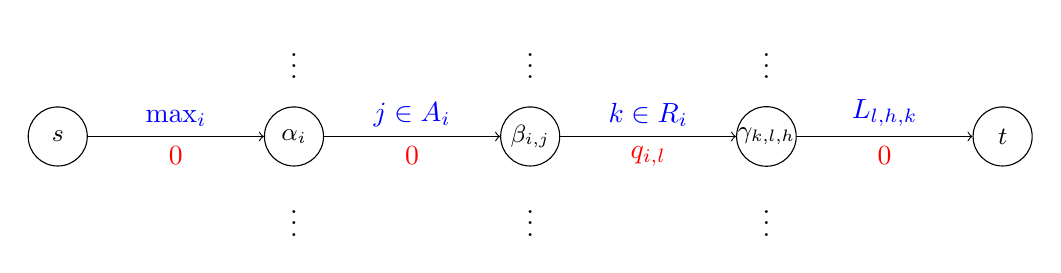
\begin{tikzpicture}

\tikzstyle{v}=[draw, circle, inner sep=0pt, font=\small, align=center, minimum size=0.75cm];
\tikzstyle{e}=[->, dashed];

\node[v] (s) at (1, 1) {$s$};
\node[v] (alpha_i) at (4, 1) {$\alpha_i$};
\node (d1) at (4, 0) {$\vdots$};
\node (d2) at (4, 2) {$\vdots$};
%\node[v] (alpha_1) at (4, 3) {$\alpha_1$};
%\node[v] (alpha_p) at (4, -1) {$\alpha_p$};

\node[v] (beta_ij) at (7, 1) {$\beta_{i, j}$};
\node (d3) at (7, 0) {$\vdots$};
\node (d4) at (7, 2) {$\vdots$};
%\node[v] (beta_11) at (7, 3) {$\beta_{1, 1}$};
%\node[v] (beta_pd) at (7, -1) {$\beta_{p, d}$};

\node[v] (gamma_klj) at (10, 1) {$\gamma_{k, l, h}$};
\node (d5) at (10, 0) {$\vdots$};
\node (d6) at (10, 2) {$\vdots$};

%\node[v] (gamma_111) at (10, 3) {$\gamma_{1, 1, 1}$};
%\node[v] (gamma_mcv) at (10, -1)  {$\gamma_{m, c, v}$};

\node[v] (t) at (13, 1) {$t$};

\draw[->] (s) to node[blue, above] {$\max_i$} node[red, below] {$0$} (alpha_i);

%\dottedarrows{{s}}{{alpha_1, alpha_p}};

\draw[->] (alpha_i) to node[blue, above] {$j \in A_i$} node[red, below] {$0$} (beta_ij);

%\dottedarrows{{alpha_1, alpha_i, alpha_p}}{{beta_11, beta_ij, beta_pd}}{alpha_i}{beta_ij};

\draw[->] (beta_ij) to node[blue, above] {$k \in R_i$} node[red, below] {$q_{i, l}$} (gamma_klj);

%\dottedarrows{{beta_11, beta_pd, beta_ij}}{{gamma_111, gamma_mcv, gamma_klj}}{beta_ij}{gamma_klj};

%\dottedarrows{{gamma_111, gamma_mcv}}{{t}};

\draw[->] (gamma_klj) to node[blue, above] {$L_{l, h, k}$} node[red, below] {$0$} (t);
\end{tikzpicture}
\end{center}

Formally, this is $G = (V, E)$, such that

\begin{align*}
  V = &\{s\} \cup \{t\}\\
      &\cup \{\alpha_i \mid i \in P\}\\
      &\cup \{\beta_{i, j} \mid i \in P, j \in S\}\\
      &\cup \{\gamma_{k, l, h} k \in R, l \in C, 1 \le h \le n(l)\}\\
  E = &\{(s, \alpha_i)\ \forall\ i\}\\
      &\cup \{(\alpha_i, \beta_{i, j}) \ \forall\ i, j \mid j \in A_i\}\\
      &\cup \{(\beta_{i, j}, \gamma_{k, l, h})\ \forall\ i, j, k, l, h \mid k \in R_i, f(l, h) = j\}\\
      &\cup \{(\gamma_{k, l, h}, t) \ \forall\ k, l, h\}
\end{align*}

with capacity function $c:E \to \Z^2$ such that
\begin{align*}
  c(s, \alpha_i) &= (0, \textstyle\max_i)\\
  c(\alpha_i, \beta_{i, j}) &= (0, j \in A_i)\\
  c(\beta_{i, j}, \gamma_{k, l, h}) &= (0, k \in R_i)\\
  c(\gamma_{k, l, h}, t) &= L_{l, h, k} = (\min(l, h, k), \max(l, h, k))
\end{align*}

where a capacity of $(a, b)$ means a lower bound of $a$ and an upper bound of $b$; and weighed by $w:E \to \mathbb{R}$, such that
\begin{align*}
  w(e) = \begin{cases}
    q_{i, l} & \text{ if } e = (\beta_{i, j}, \gamma_{k, l, h})\\
    0 & \text{otherwise}
  \end{cases}
\end{align*}

This solves the problem in a similar way as the single course day. A unit of flow going through $(\alpha_i, \beta_{i, j})$ repersents professor $i$ working on the $j$th day. If this unit flows through $(\beta_{i, j}, \gamma_{k, l, h})$, this represents working as the $k$th role on the $h$th class of the $l$th course.

The constraints on the outgoing flow for $\gamma_{k, l, h}$ imply that the only way to obtain a flow of $\sum_{k, l, h} n_{k, l, h}$ units is that each outgoing edge is saturated. Thus a maximum flow of that magnitude is equivalent to a valid assignment of professors to roles in each class of each course.

Furthermore, we wish to maximize the quality of each professor teaching each course. This means maximizing the sum of the $q_{i, l}$, since this represents that the $i$th professor is teaching a class of the $l$th course. Thus among these maximum flows, we want the one of maximum cost.

Since this problem is solvable in polynomial time in the number of nodes and edges of the network, and in our case these are also in $O(poly(p, d, m, v, c))$, the problem is solvable in polynomial time, and thus is also in \textsc{P}.


\subsection{As a maximum-weight perfect bipartite matching}
Again in the case where professors have no upper bound on the number of classes they can teach, and the role requirements for each class have the same upper and lower bounds, we can view this restriction a maximum-weight perfect matching on a bipartite graph. The construction is similar to the single course case:

\begin{center}
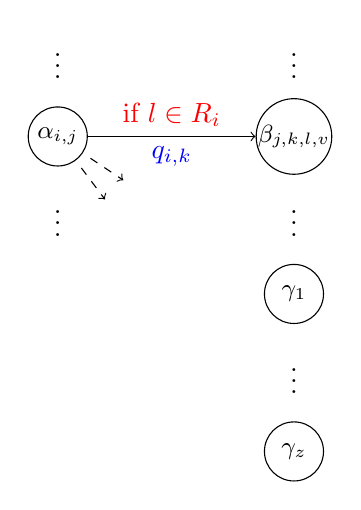
\begin{tikzpicture}
  %\node[v] (a11) at (0, 4) {$\alpha_{1, 1}$};
  \node (d1) at (0, 3) {$\vdots$};
  \node[v] (aij) at (0, 2) {$\alpha_{i, j}$};
  \node (d2) at (0, 1) {$\vdots$};
  %\node[v] (ant) at (0, 0) {$\alpha_{p, d}$};

  %\node[v] (b1111) at (3, 4) {$\beta_{1, 1, 1, 1}$};
  \node (d3) at (3, 3) {$\vdots$};
  \node[v] (bjklv) at (3, 2) {$\beta_{j, k, l, v}$};
  \node (d4) at (3, 1) {$\vdots$};
  %\node[v] (btcmncm) at (3, 0) {$\beta_{d, c, m, n'_{c, m}}$};

  \node[v] (c1) at (3, 0) {$\gamma_1$};
  \node (d5) at (3, -1) {$\vdots$};
  \node[v] (cz) at (3, -2) {$\gamma_z$};

  \draw[->] (aij) to node[above, red] {if $l \in R_i$} node[below, blue] {$q_{i, k}$} (bjklv);
  \dottedarrows{{aij}}{{bjklv, c1, cz}}{aij}{bjklv};
\end{tikzpicture}
\end{center}

Formally, we have a graph $G = (V, E)$, where

\begin{align*}
  V = & \{\alpha_{i, j} \mid 1 \le i \le p, 1 \le j \le d, j \in A_i\}\\
    & \cup \{\beta_{j, k, l, v} \mid 1 \le j \le d, 1 \le k \le c, 1 \le l \le m, 1 \le v \le n'_{c, l}\}\\
    & \cup \{\gamma_i \mid 1 \le i \le z\}\\
  E = & \{\{\alpha_{i, j}, \beta_{j, k, l, v}\}\ \forall\ i, j, k, l, v, l \in R_i\}\\
      & \cup \{\{\alpha_{i, j}, \gamma_k\} \mid \ \forall\ i, j, k\}
\end{align*}

where we have defined, as before, $x = \sum_{i = 1}^p |\{j \mid 1 \le j \le d, a_{i, j} = 1\}|$, $y = \sum_{k = 1}^c \sum_{l = 1}^m n'_{k, l}$, and $z = x - y$.

We also have a cost function $w:E \to \mathbb{R}$, such that:

\begin{align*}
  w(\alpha_{i, j}, \beta_{j, k, l, v}) &= q_{i, k}\\
  w(\alpha_{i, j}, \gamma_k) &= 0
\end{align*}

Conceptually, we see this as assigning proffesors $i$, on day $j$, to either teach the $k$th course, on the $l$th role (being the $v$th instance of this role for that class), or to have a ``holiday'', when they're assigned to some $\gamma$. The cost of assigning a professor to teach a class is the quality the professor has for that class, hence what we want to maximize is the sum of the costs of the professor assignments in this bipartite graph.

This formulation again provides us with an integer linear programming formulation, noting by $B$ the incidence matrix of $G$:

\begin{alignat*}{2}
  \text{maximize }   & q^t x \\
  \text{subject to } & Bx \le \mathbf{1}\\
                     & x ge \mathbf{0}\\
                     & x \in \mathbb{Z}^M
\end{alignat*}

which, by unimodularity of $B$ since $G$ is bipartite,  has an integral linear relaxation:

\begin{alignat*}{2}
  \text{maximize }   & q^t x \\
  \text{subject to } & Bx \le \mathbf{1}\\
                     & x \ge \mathbf{0}\\
                     & x \in \mathbb{R}^M\\
\end{alignat*}

and thus an optimal solution can be found in polynomial time in the size of $B$, which by our construction of $G$ is in $O(poly(p, t))$.

\end{document}
